\begin{figure}[th]
\centering
\subfloat[A$\rightarrow$D]{
	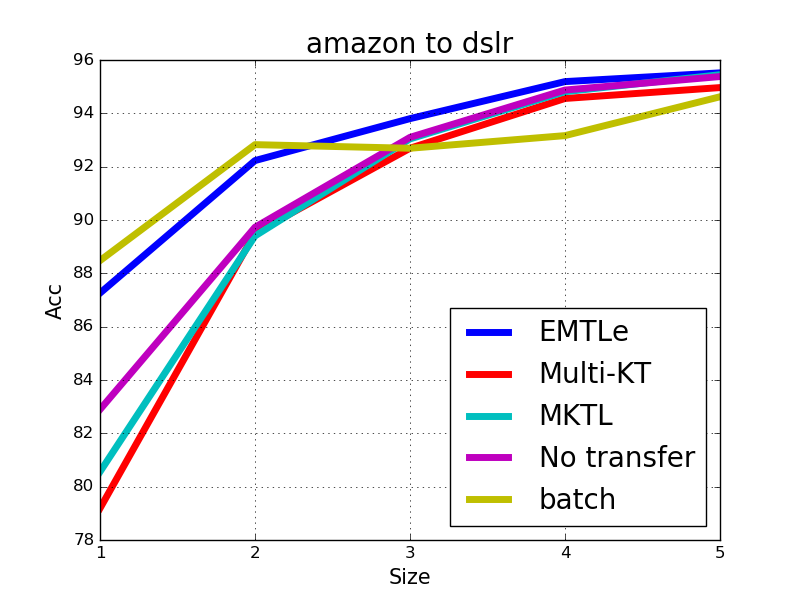
\includegraphics[width=0.45\textwidth]{pakdd/fig/amazontodslr.png}\label{g}
}
\subfloat[C$\rightarrow$D]{
	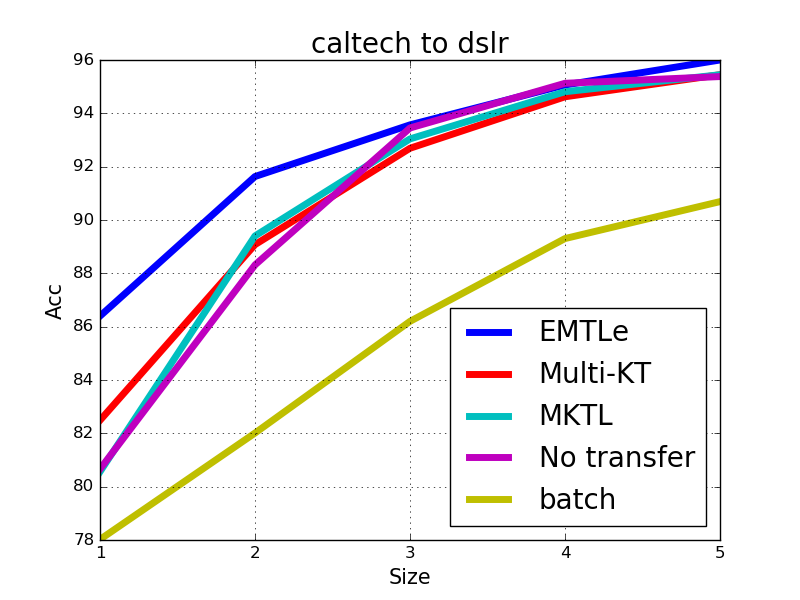
\includegraphics[width=0.45\textwidth]{pakdd/fig/caltechtodslr.png}\label{h}
}\\
\subfloat[W$\rightarrow$D]{
	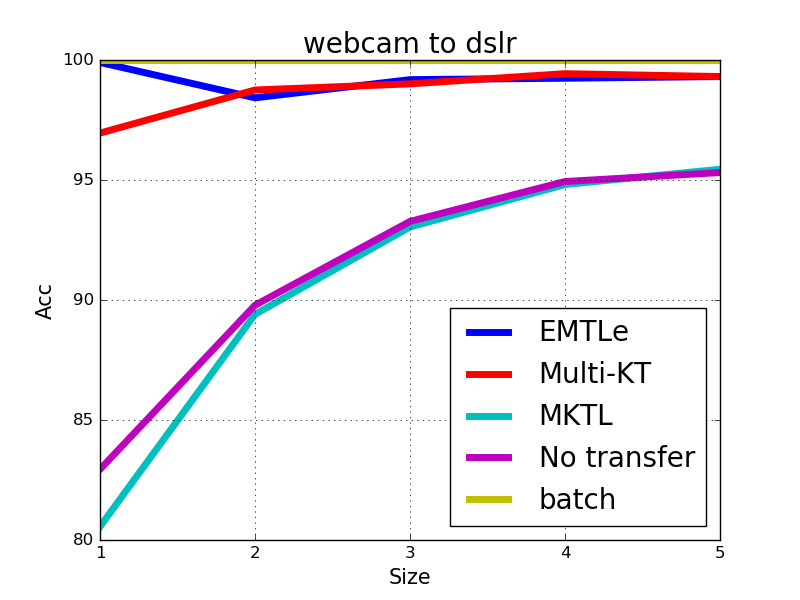
\includegraphics[width=0.45\textwidth]{pakdd/fig/webcamtodslr.png}\label{i}
}
\subfloat[A$\rightarrow$W]{
	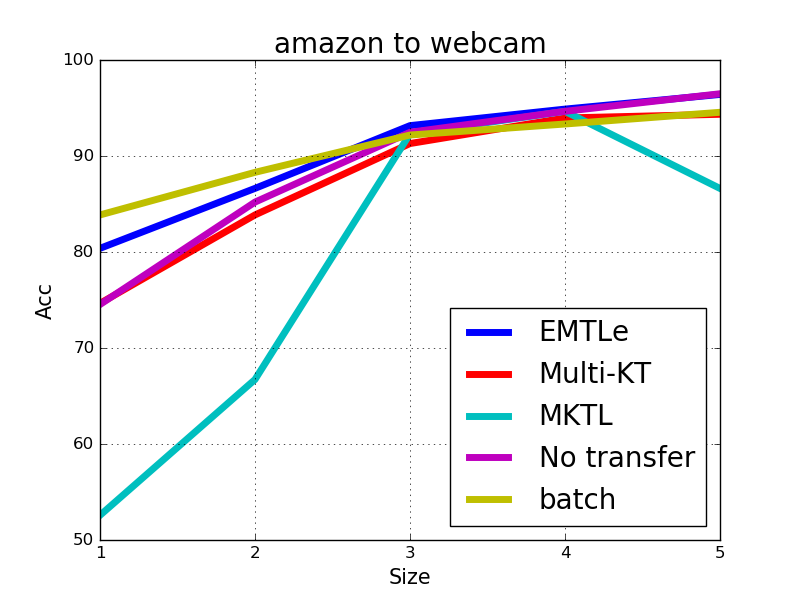
\includegraphics[width=0.45\textwidth]{pakdd/fig/amazontowebcam.png}\label{j}
}\\
\subfloat[C$\rightarrow$W]{
	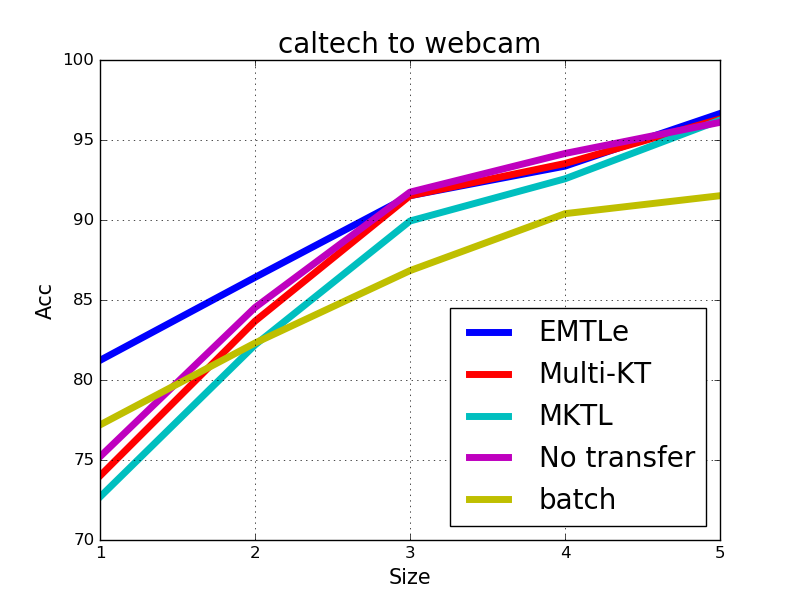
\includegraphics[width=0.45\textwidth]{pakdd/fig/caltechtowebcam.png}\label{k}
}
\subfloat[D$\rightarrow$W]{
	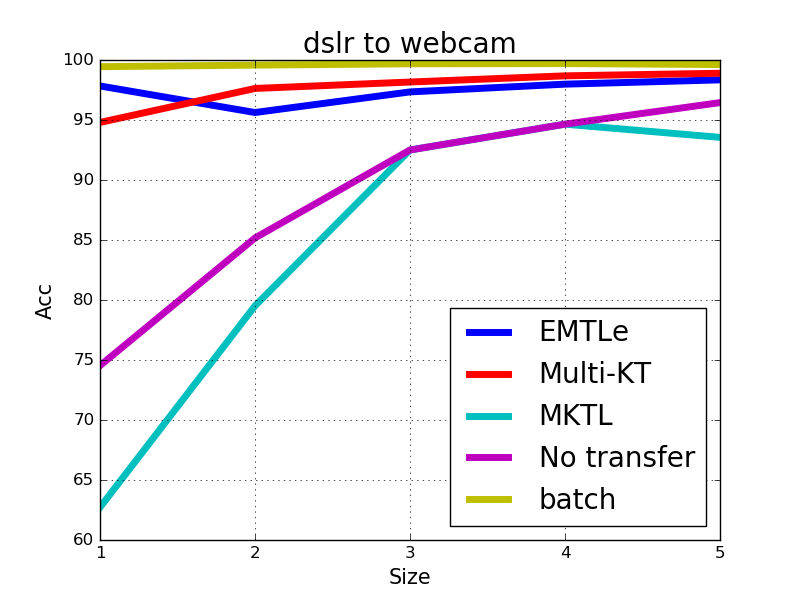
\includegraphics[width=0.45\textwidth]{pakdd/fig/dslrtowebcam.png}\label{l}
}
\caption{Recognition accuracy for HTL domain adaptation from a single source (Part1). 5 different sizes of target training sets are used in each group of experiments. A, D, W and C denote the 4 subsets in Table \ref{tab:class_info} respectively.}
\label{fig:exp}
\end{figure}


\begin{figure}[th]
	\centering
	\subfloat[C$\rightarrow$A]{
		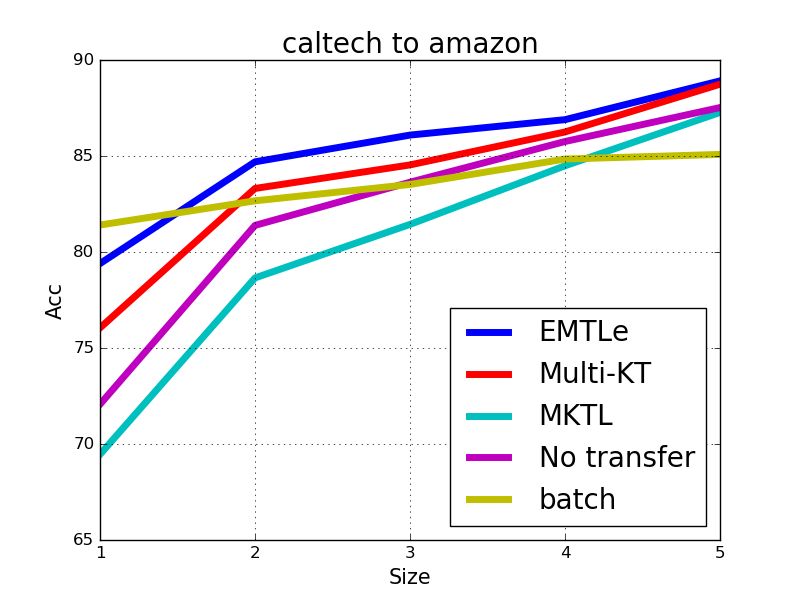
\includegraphics[width=0.45\textwidth]{pakdd/fig/caltechtoamazon.png}
	}
	\subfloat[D$\rightarrow$A]{
		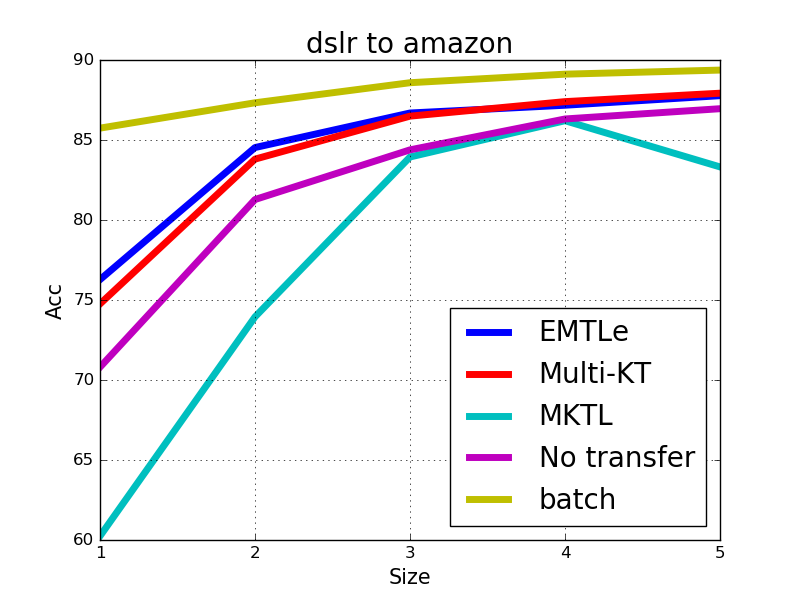
\includegraphics[width=0.45\textwidth]{pakdd/fig/dslrtoamazon.png}
	}\\
	\subfloat[W$\rightarrow$A]{
		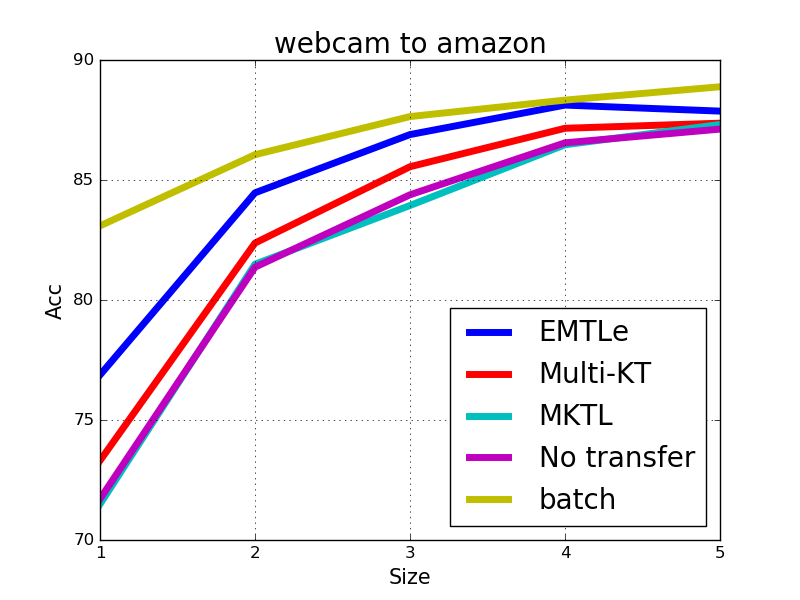
\includegraphics[width=0.45\textwidth]{pakdd/fig/webcamtoamazon.png}
	}
	\subfloat[A$\rightarrow$C]{
		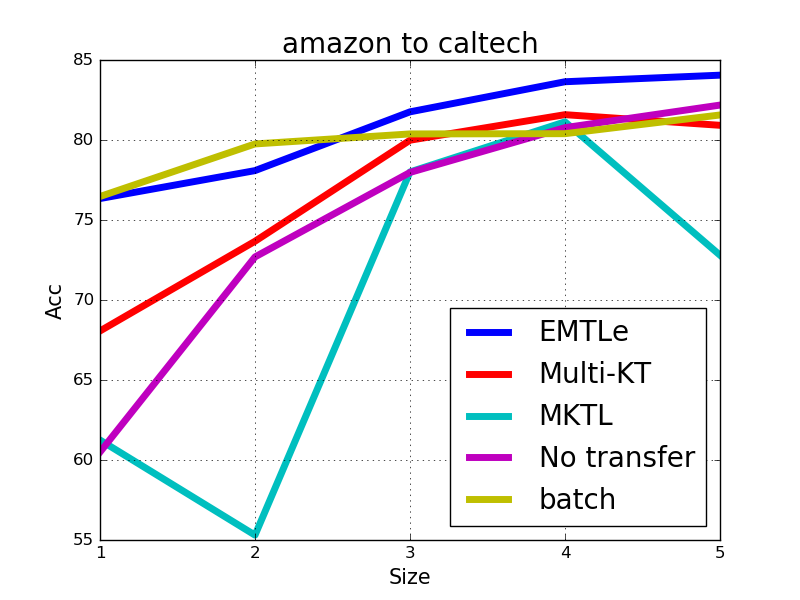
\includegraphics[width=0.45\textwidth]{pakdd/fig/amazontocaltech.png}
	}\\
	\subfloat[D$\rightarrow$C]{
		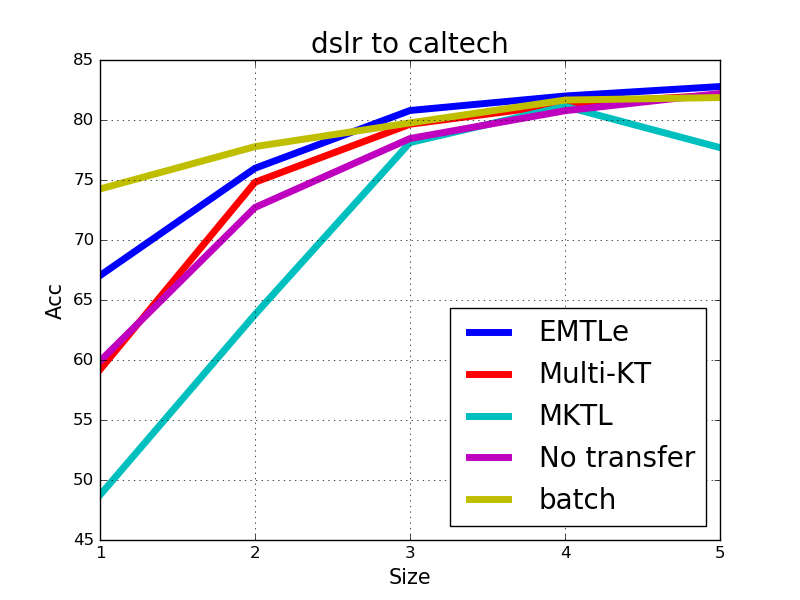
\includegraphics[width=0.45\textwidth]{pakdd/fig/dslrtocaltech.png}
	}
	\subfloat[W$\rightarrow$C]{
		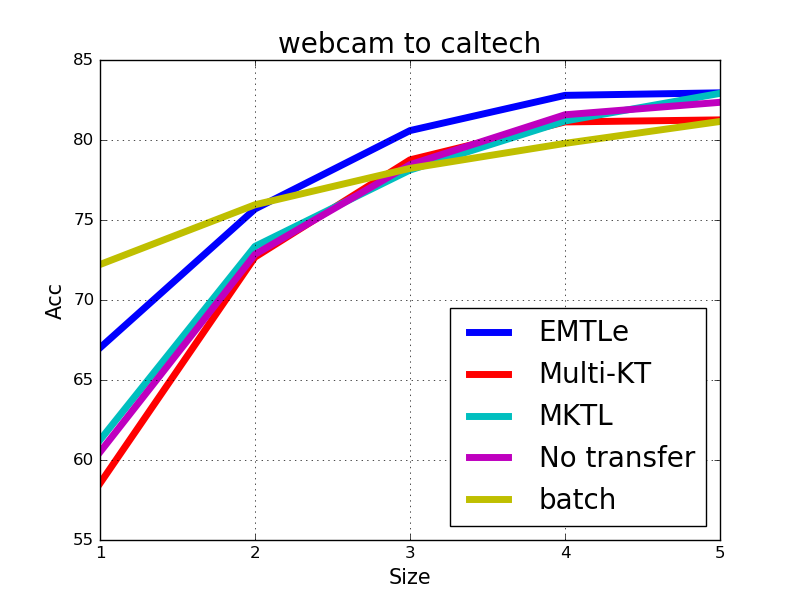
\includegraphics[width=0.45\textwidth]{pakdd/fig/webcamtocaltech.png}
	}\\
	\caption{Recognition accuracy for HTL domain adaptation from a single source (Part2). 5 different sizes of target training sets are used in each group of experiments. A, D, W and C denote the 4 subsets in Table \ref{tab:class_info} respectively.}
\end{figure}
\textbf{Observation \& discussion:} EMTLe can significantly outperform other baselines especially with a small training set. %Moreover, in some groups of experiments, they even suffer from negative transfer on the small training set. 
As we have discussed above, when the training set is small, with the transfer parameter estimated by our $\ell_2$ penalty in our high-level objective functions, EMTLe has a strong generalization ability and performs better on the test data. As the training size increases, the variance of training data decreases and the affect of the $\ell_2$ penalty term become less significant. Therefore, EMTLe and the other two HTL baselines show similar performance. 
It is interesting to see that MKTL even falls into negative transfer even with 5 training examples per class in some experiments. We found that, MKTL is more sensitive to the variance of the training data. Its performance is not as stable as Multi-KT and EMTLe over the 10 experiments. Because MKTL needs to learn more hyperparameters than Multi-KT and EMTLe, even though the training size increases, it may not be able to obtain a good model. 
In some experiments, we can see that EMTLe can even outperform the Batch method which can access more information and is expected to outperform the other methods under the setting of HTL.